\chapter[Systematic Mapping Study of Tag Cloud Research]{Systematic Mapping Study\\of Tag Cloud Research}

\label{chap:strateval}
\ifpdf
    \graphicspath{{Chapters/SystematicMappingStudy/SystematicMappingStudyFigs/PNG/}{Chapters/SystematicMappingStudy/SystematicMappingStudyFigs/PDF/}{Chapters/SystematicMappingStudy/SystematicMappingStudyFigs/}}
\else
    \graphicspath{{Chapters/SystematicMappingStudy/SystematicMappingStudyFigs/EPS/}{Chapters/SystematicMappingStudy/SystematicMappingStudyFigs/}}
\fi


Information visualisation techniques can be challenging to evaluate \citep{plaisant04}. This is because, in addition to general evaluation challenges (such as choosing appropriate questions and tasks, defining methods and then executing the evaluation correctly) the visualisation focus on the data exploration process is difficult to capture and quantify. We embarked on a systematic mapping study of previous research evaluating the tag cloud technique or interactive tools that included tag cloud visualisation. This study identified topics, fields or domains that had not been extensively researched, and approaches and methods which had been used for evaluation. To classify our work, we used a set of information visualisation guiding scenarios which are outlined in \S\ref{sect:strategies}. Research questions and goals for the study are presented in \S\ref{sect:researchquestions}. The research methodology including data sources, study selection and data extraction are outlined in \S\ref{sect:mappingmethods}. Results for research topic, methods, domains and approaches are discussed in \S\ref{sect:mappingresults}. Finally, summary and conclusions are presented in  \S\ref{sect:mappingdiscussion} and \S\ref{sect:mappingconclusions}. 

%This work provided an overview of what is known about tag clouds, and helped us plan and focus our overall evaluation strategy.

\section{Strategies for evaluation}\label{sect:strategies}

In 2012, \citet{lam12} identified seven guiding scenarios for information visualisation evaluation. These scenarios were gathered from a systematic review of 803 information visualisation papers (345 of which included evaluations). Of these scenarios, four can be roughly defined as evaluation of the \emph{data analysis process} (EWP, VDAR, CTV, CDA -- described in \S\ref{sect:dataextraction}) and the remaining three evaluate the \emph{visualisation use} (UP, UE, VA). These two types of strategies have different goals and use different methodologies. 

Evaluation of the \emph{data analysis process} has a goal of understanding the underlying process and roles played by the visualisation itself, and captures a more whole-tool holistic view. The results from this type of analysis may be more meaningful as realistic tasks and scenarios are used. However, results can be more difficult to quantify. Also, the whole tool is evaluated so evaluation may require full featured and mature tool.

The \emph{visualisation use} type strategies do not evaluate the whole tool but a system slice or technique. They are used to evaluate design decisions, explore the design space, benchmark existing systems or test usability. For these strategies, outputs are easier to quantify generated insight. There is a need to break the evaluation into techniques or visual encoding types, so careful prioritisation is needed. Because of this breaking off into sections, more than one experiment may be needed. Tasks may also need to be heavily abstracted which impacts realism.

In the systematic review performed by \citet{lam12}, only 15 percent of papers used data analysis process type strategies in their evaluation. They concluded that evaluation in the information visualisation sector has been following in the footsteps of evaluations for Human Computer Interaction (HCI) and Computer Graphics (CG), both of which are traditionally focused on controlled experiments and usability evaluations. The data process strategy research questions (such as a tools support for reasoning, knowledge discovery or decision making) are of high relevance and practical value. \citet{lam12} highlighted the need to think critically about the goals of the types of evaluations needed for information visualisation.

We were interested to find out what types of evaluations had been performed for tools utilising tag cloud visualisation techniques, and what research topics and domains the evaluations focused on so we performed a systematic mapping study on 60 selected primary studies from 2007 to 2012. 

%We found that 93\% of evaluations used visualisation use type strategies. This was despite 43\% of papers incorporating tag clouds (or enhanced tag clouds) into interactive systems which likely had goals of exploring data or discovering information. Research was strongly focussed in the WWW domain. 

\section{Systematic mapping study}\label{sect:researchquestions}

We had a number of goals for our systematic mapping study. We wanted to find all papers which have evaluated the effectiveness of the tag cloud visualisation technique in order to identify those areas of tag cloud visualisation which contain either exhaustive research (allowing us to apply and build on), or deserts of information (allowing us to shape future research in this area). Secondly, tag clouds are most commonly associated with the web - we were interested to find out what other domains had proposed and evaluated tag cloud visualisation techniques. Finally, we wanted to discover what evaluation approaches and methods had been used by tag cloud evaluation studies in order to achieve their research goals. Overall, the systematic mapping study should serve to build an overview of what is known about tag clouds as a visualisation technique in general, identifying clusters of evidence and establishing areas of research where knowledge gaps exist. 

\begin{description}
\item[RQ:] \textit{What topics for tag cloud visualisation have been evaluated and to what extent?} We want to establish which topic areas have been focused on in previous research, in order to help shape future research.
\item[RQ:] \textit{What evaluation approaches and methods have been used?} We want to discover what types of evaluation have been undertaken for tag cloud visualisation, and what methods were used.
\item[RQ:]\textit{ For which fields or domains have tag cloud visualisations been evaluated?} The domain which tag clouds are primarily associated with is the web. We want to know what other fields or domains tag cloud visualisation has been proposed and evaluated for. 
\end{description}


%\section{Research Questions}\label{researchquestions}
%\input{Chapters/SystematicMappingStudy/researchquestions}

\section{Methods}\label{sect:mappingmethods}
%Scope of the study is as follows:
%\begin{itemize}
%\item Population: Published scientific literature reporting on information visualisation.
%\item Intervention: Research including an evaluation of tag cloud visualisation.
%item Outcomes of relevance: Quantity and type of evidence relating to tag clouds as a visualisation or user interface.
%\item Experimental design: Any scientific experiment or empirical study.
%\end{itemize}
During the course of the systematic mapping study, the following activities were carried out: define research questions, define data sources and search strategy, perform searches in all designated digital libraries and search engines using the filter, remove duplicate studies (results reported from multiple search engines), review each paper using specified inclusion/exclusion criteria and determine relevance to the topic and research questions, perform data extraction, and perform data synthesis.

\subsection{Data sources and search strategy}

The digital libraries and search engines which were used to extract the articles were ACM digital library\footnote{\url{dl.acm.org/}},  IEEE Explore\footnote{\url{ieeexplore.ieee.org}}, SpringerLink\footnote{\url{www.springerlink.com}}, CiteSeer\footnote{\url{citeseerx.ist.psu.edu/}}, Scopus\footnote{\url{www.scopus.com}}, Sage Journals\footnote{\url{online.sagepub.com/}}, Scirus\footnote{\url{www.scirus.com}}, Web of Science\footnote{\url{wokinfo.com/}}, ScienceDirect\footnote{\url{www.sciencedirect.com/}} and arXiv\footnote{\url{arxiv.org/}}.

The search terms were grouped into three categories 1) pertaining to visualisation technique 2) relating to visualisation type and 3) search terms relating to evaluation.

\pagebreak

\begin{verbatim}
("tag cloud" OR "tag clouds" OR "tagcloud" OR "tagclouds") AND
("evaluation" OR "qualitative" OR "quantitative"
OR "experiment" OR "experimentation" OR "experiments"
OR "study" OR "studies") AND 
("visualisation" OR "visualization" OR 
"user interface" OR "user interfaces")
\end{verbatim}

These search groups were joined together with the use of a boolean AND to search document metadata (where available) such as title, abstract, classification and keywords. Additionally, each query had to be adapted according to the interface and query specification of the search engine.

In order to validate the search strategy, a check was performed to ensure a small sample of papers (12) was included in the search results \citep[][]{bateman08, hearst08, kaser07, lohmann09, oosterman10, rivadeneira07, schrammel09, schrammel09b, seifert08, kuo07, halvey07, sinclair08}. These papers had previously been noted as relevant to the research questions during an initial review of the literature.

\subsection{Primary study selection}
Each paper returned from the digital libraries and search engines using the specified query was checked for duplication against other database results. An initial result total of 181 was whittled down to 100 after removal of duplicates (see Table~\vref{tab:searchresults1}).

\begin{table}
\centering
\caption{\textit{Initial search results from digital libraries and corresponding duplicates}}
\begin{tabular}{|l|c|c|c|} \hline
\textbf{Digital Libraries}&\textbf{Results}&\textbf{Duplicates}&\textbf{Total}\\ \hline
ACM digital library&16&1&15\\ \hline
IEEE Explore&38&0&38\\ \hline
SpringerLink&10&0&10\\ \hline
CiteSeer&2&2&0\\ \hline
Scopus&70&55&15\\ \hline
Sage Journals&2&2&0\\ \hline
Scirus&0	&0&0\\ \hline
Web of Science&40&19&21\\ \hline
ScienceDirect&2&2&0\\ \hline
arXiv&1&0&1\\ \hline
\textbf{Totals}&\textbf{181}&\textbf{81}&\textbf{100}\\
\hline\end{tabular}
\label{tab:searchresults1}
\end{table}

Each paper was then checked for relevancy using the title, abstract and keywords. Studies that met one of the following inclusion criteria were included: 

\begin{itemize}
\item studies describing the evaluation of tag cloud visualisation
\item studies describing the evaluation of a visualisation or user interface based on the tag cloud technique
\item studies describing the evaluation of a system which utilises tag cloud visualisation 
\item studies describing the evaluation of a system which utilises a visualisation or user interface based on the tag cloud technique
\end{itemize}

Studies that met one of the following exclusion criteria were excluded:

\begin{itemize}
\item studies where only an abstract was available
\item studies where the paper was not available in English
\item studies describing the evaluation of a system where the evaluation method did not specifically include the tag cloud component
\item studies where the described evaluation served as a proof of concept
\item duplicate articles of the same study from different sources
\end{itemize}

In many cases it was not possible to determine relevancy of the study from the abstract alone, particularly in determining whether the evaluation method actually included evaluation of the tag cloud component of a system. For these studies, it was necessary to consider the paper as a whole. Each paper was reviewed twice for inclusion/exclusion criteria, during two passes of the search results as a means of validation. During the second review of the paper, a set of keywords was extracted. These served as the basis for the creation of the classification categories within mapping facets.

During the inclusion/exclusion phase a further 40 documents were excluded from the study, bringing the total number of primary papers included to 60 (see Table~\vref{tab:searchresults2} for the exclusion details, after duplicates had been removed).

\begin{table}
\centering
\caption{\textit{Search results from digital libraries and corresponding excluded papers}}
\begin{tabular}{|l|c|c|c|} \hline
\textbf{Digital Libraries}&\textbf{Results}&\textbf{Excluded}&\textbf{Total}\\ \hline
ACM digital library&15&1&14\\ \hline
IEEE Explore&38&22&16\\ \hline
SpringerLink&10&4&6\\ \hline
Scopus&15&8&7\\ \hline
Web of Science&21&5&16\\ \hline
arXiv&1&0&1\\ \hline
\textbf{Totals}&\textbf{100}&\textbf{40}&\textbf{60}\\
\hline\end{tabular}
\label{tab:searchresults2}
\end{table}

\subsection{Data extraction}\label{sect:dataextraction}

For each research question, a set of classification categories was devised within a mapping facet.

For RQ \textit{Research topic}, we determined the categories by extracting keywords from the primary studies:

\begin{itemize}
\item evaluating the effectiveness of the tag cloud technique
\item determining perceived physical demand or workload
\item proposal of evaluation metrics or methodologies
\item making design guidelines or recommendations
\item determining support for user process (social navigation, incidental learning, reflections of learners, determining credibility of sources, dynamic representation of places/situations)
\item discovering limits of visual perception (visual features or properties, layout)
\item determining user motivation for use
\item proposal of a tag cloud enhancement (with respect to relationships, topic clustering, temporal evolution, tag ranking algorithms, tagging interfaces, interfaces for a special dataset or medium, layout optimisation)
\item evaluations of systems/visualisations targeting a special population (Chinese readers, Hebrew readers, tools for the blind)
\end{itemize}

For RQ \textit{Evaluation approaches and methods}, the Seven Guiding Scenarios for Information Visualisation Evaluation proposed by \citet{lam12} were used to classify the evaluation approaches and methods:

\begin{description}
\item[EWP:] \emph{Understanding Environments and Work Practices.} Studying the design context for visualisation tools including tasks, work environments, and current work practices. Types of research methods include field observation, interviews and laboratory observation.
\item[VDAR:] \emph{Evaluating Visual Data Analysis and Reasoning.} Discovering if and how a visualisation tool supports the generation of actionable
and relevant knowledge in a given domain. Types of research methods include case studies and controlled experiments.
\item[CTV:] \emph{Evaluating Communication Through Visualisation.} Discovering if and how communication can be supported by visualisation (for example through learning, teaching, idea presentation and casual consumption of ambient displays). Types of research methods include controlled experiments and field observation and interviews. 
\item[CDA:] \emph{Evaluating Collaborative Data Analysis.} Studying whether a tool allows for collaboration, collaborative analysis, and/or collaborative decision-making processes. Types of research methods include heuristic evaluation, log analysis and field or laboratory observation.
\item[UP:] \emph{Evaluating User Performance.} Studying if and how specific visualisation features affect objectively measurable user performance. Types of research methods include controlled experiments and field logs.
\item[UE:] \emph{Evaluating User Experience.} People's subjective feedback and opinions.  Types of research methods include informal evaluation, usability tests and field observation.
\item[VA:] \emph{Evaluating Visualisation Algorithms.} Study the performance and quality of visualisation algorithms by judging the generated output. Types of research methods include algorithmic performance measurement and quality metrics.
\end{description}

By classifying the studies based on these guiding scenarios we get a picture of the underlying evaluation goals, rather than just a description of the type of research methods employed. 

For RQ \textit{Visualisation domain}, the categories were again determined by keywords we extracted from the primary studies:

\begin{itemize}
\item web (user generated content, database search results, recommendation systems)
\item mixed media (image, film, television and audio)
\item software engineering
\item text corpora
\item geographical information
\item mobile phone
\item digital forensics
\item health and medicine (online forums, tool for the blind)
\item situated displays
\item database search results (OLAP, online database)
\item multi-variate data
\end{itemize}

Papers may cover more than one domain or topic so can be associated with multiple classification types. Where applicable, papers were categorised into sub-topics (as indicated within the brackets).


\section{Results}\label{sect:mappingresults}

The distribution of primary papers over time can be seen in Figure~\vref{fig:barchart1} --- papers span from 2007 to 2012 (the mapping study was conducted 2012). Figure~\ref{fig:bubble1} shows a bubble chart of the mapping facets research topic and evaluation method. The totals do not match exactly with the total number of papers included in the study as it is possible for papers to cover both multiple topics and use multiple evaluation methods within the study. This is particularly common where studies use the evaluation approach UP (measuring user performance) as this evaluation method tends to use controlled studies and a corresponding UE (user evaluation) component, such as a lab questionnaire requesting subjective user feedback. It is possible to see in this chart a heavy tendency towards UP and UE evaluation approaches within the domains of text corpora and web. The focus on web and text is not surprising as these are the domains where tag clouds are most commonly found.

\begin{figure}[!htb]
\centering
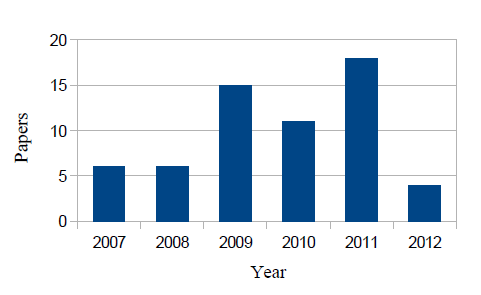
\includegraphics{barchart1.png}
\caption{\textit{Distribution of papers over time}}
\label{fig:barchart1}
\end{figure}

\begin{figure}[!htb]
\centering
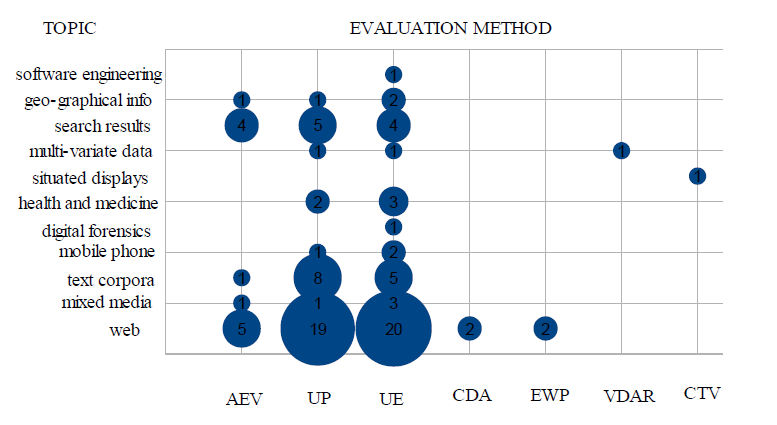
\includegraphics[scale=0.75]{bubble1.png}
\caption{\textit{Mapping facets: research topic and evaluation method}}
\label{fig:bubble1}
\end{figure}

\subsection{Research topic}\label{topic}

A breakdown of the numbers of studies found in each research topic and sub-topic can be found in Table~\vref{tab:researchtopic}. The research topics were heavily skewed towards evaluations of proposed enhancements to tag clouds (see Figure~\vref{fig:pie1}). The most commonly proposed type of enhancement was to cater for a special dataset or medium \citep[such as][]{aras09, kim09, kurtz11, shrinivasan09} where interfaces were built for domains such as geo-graphical information, mobile phone, software engineering or multi-variate data. Other popular topics were proposals for improving perceived tag cloud visualisation shortcomings, such as determining relationships and displaying temporal evolution \citep[for example][]{DiCaro2011120, gomez11}. Only two papers proposed design guidelines or recommendations \citep{rivadeneira07, bateman08}. Evaluations of effectiveness and determining the limits of visual perception made up 22 percent of papers. Tag cloud support was researched by 6 percent of papers for a particular user process.

\begin{landscape}
\begin{table}
\centering
\caption{\textit{Results for the research topic}}
\begin{tabular}{|l|c|p{6cm}|x{2cm}|} \hline
\textbf{Topic}&\textbf{Number}&\textbf{Sub-topic}&\textbf{Number}\\ \hline
Proposal of a tag cloud enhancement&
41&
\parbox[t]{7cm}{\raggedright relationships\break  topic clustering\break temporal evolution\break tag ranking algorithms\break tagging interfaces\break  interface for a special dataset\break interface for a special medium\break layout optimisation}&
7\par 6\par 4\par 9\par 2\par 13\par 2\par 5\\
%relationships\par  topic clustering\par  temporal evolution\par tag ranking algorithms\par tagging interfaces\par  interface for a special dataset\par interface for a special medium\par layout optimisation&7\par 6\par 4\par 9\par 2\par 13\par 2\par 5\\ 
Proposal of evaluation metrics or methodologies&2&&\\
Evaluating the effectiveness of the tag cloud technique&9&&\\
Discovering limits of visual perception&8&visual features or properties\par layout&5\par 3\\
Making design guidelines or recommendations&2&&\\
Determining user motivation for use&3&&\\
Determining support for user process&6&social navigation\par incidental learning\par reflections of learners\par determine credibility of sources\par dynamic representation of places&1\par 1\par 1\par 1\par 1\\
Determining perceived physical demand or workload&2&&\\
Evaluations of systems targeting a special population&4&\par Chinese readers\par Hebrew readers\par tools for the blind&2 \par 1\par 1\par\\
\hline\end{tabular}
\label{tab:researchtopic}
\end{table}
\end{landscape}

\begin{figure}[!htb]
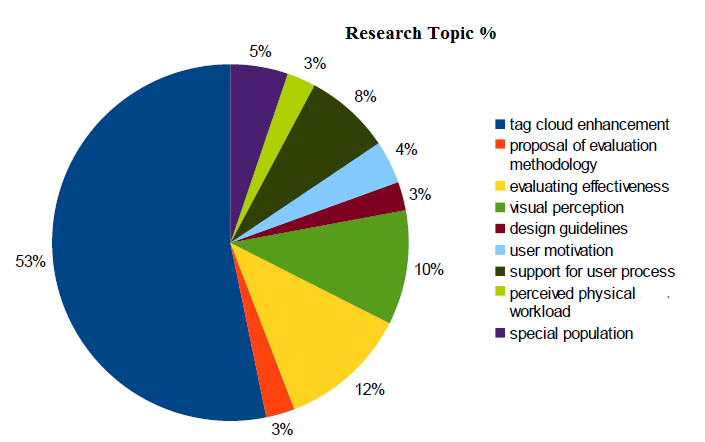
\includegraphics[scale=0.75]{pie1.png}
\caption{\textit{Research topic as a percentage of total papers included in the study}}
\label{fig:pie1}
\end{figure}

\subsection{Research approach and methods}

Table~\vref{tab:evaluation} shows results for research approach and method. By far the most popular methods of evaluation were the `User Performance' and `User Experience' categories, closely followed by `Automated Evaluation of Visualisation' (for brevity these shall be referred to elsewhere as UP, UE and AEV). These three evaluations strategies make up one of the two main categories of evaluation strategies referred to as `visualisation use'. They represent a total of 93 percent of papers surveyed. This is consistent with the findings of \citet{lam12}, where 85 percent of evaluations in information visualisation papers surveyed were representative of these categories. This was thought to be a possible by-product of the traditions in Human Computer Interaction (HCI) and Computer Graphics (GC) which historically have focused on evaluation by controlled experiment, usability and algorithm evaluation. 

All UP category papers reviewed in this study performed controlled experiments, and the vast majority of evaluations within the UE category were carried out via lab questionnaires. 

\begin{table}
\centering
\caption{\textit{Results for the research approach and method}}
\begin{tabular}{|p{2cm}|x{2cm}|p{5cm}|x{2cm}|} \hline
\textbf{Approach}&\textbf{Number}&\textbf{Method}&\textbf{Number}\\ \hline
AEV	&14&algorithm perfomance\par quality metrics&13\par 5\\
UP&32&controlled experiments&32\\
UE&35&informal evaluation\par usability test\par lab questionnaire&3\par3\par30\\
CDA&2&log analysis&2\\
EWP&2&interviews&2\\
VDAR&1&case study&1\\
CTV	&1&field observation\par interviews&1\par1\\
\hline\end{tabular}
\label{tab:evaluation}
\end{table}

\subsection{Visualisation domain}

Visualisation domain category results are found in Table~\vref{tab:domain}. Nearly half of all visualisation domains pertained to the web, with a significant portion of those relating to user generated content \citep[for example][]{bateman08, halvey07, kaser07, skoutas11}. Furthermore, another 11 percent of all domains evaluated visualisations of text corpora. This is understandable given tag cloud visualisation web-based beginnings, and visualisation of label identifiers and textual data is a key advantage of tag clouds. However, it should be possible to apply an information visualisation technique  such as this to any domain where textual data exists. Database search results, particularly for online databases, were another popular domain of research \citep{Wilson11, yamamoto09}.

\begin{table*}
\centering
\caption{\textit{Results for the visualisation domain}}
\begin{tabular}{|l|c|p{5cm}|x{2cm}|} \hline
\textbf{Domain}&\textbf{Number}&\textbf{Sub-domain}&\textbf{Number}\\ \hline
Web&33&user generated content\par database search results\par  recommendation systems&25\par 7 \par 1\\
Mixed media&4&image\par film \par television\par audio&1\par 1\par 1\par 1\\
Text corpora&9&&\\
Mobile phone&2&&\\
Digital forensics&1&&\\
Health and medicine&3&online forums\par tools for the blind&1\par 1\\
Situated displays&1&&\\
Multi-variate data&2&&\\
Database search results&9&online database\par OLAP&7\par 2\\
Geographical information&3&&\\
Situated displays&1&&\\
Software engineering&1&&\\
\hline\end{tabular}
\label{tab:domain}
\end{table*}

\begin{figure}[!htb]
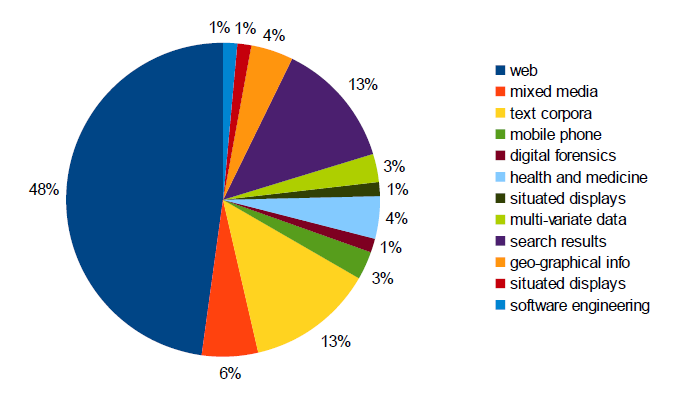
\includegraphics[scale=0.75]{pie2.png}
\caption{\textit{Visualisation domain as a percentage of total papers included in the study}}
\label{fig:pie2}
\end{figure}


\section{Summary and discussion}\label{sect:mappingdiscussion}

We wanted to build an overview of what was known about tag clouds as a visualisation technique in general, identifying clusters of evidence and establishing areas of research where knowledge gaps existed. We identified 60 papers spanning from 2007 to 2012 which were relevant to this evaluation of tag cloud visualisation evaluation. 

\begin{description}

\item[RQ:] \textit{What topics for tag cloud visualisation have been evaluated and to what extent?} Topics and total number of papers are found in Table~\vref{tab:researchtopic}. We wanted to find all papers which have evaluated the effectiveness of the tag cloud visualisation technique  so we could identify relevant research that might be applied and built upon, or areas where information was sparse. Only nine papers evaluated the effectiveness of tag cloud visualisation. While this can be widened to 16 to include papers which discuss issues surrounding the visual perception of tag clouds, this indicates there is still room to define the overall effectiveness of tag clouds as a technique. There was a large proportion of papers (43 percent) evaluating interactive interfaces for special datasets, mediums or populations. 

\item[RQ:] \textit{What evaluation approaches and methods have been used?} Evaluation approaches and total number of papers are found in Table~\vref{tab:evaluation}. We wanted to discover what types of evaluation have been undertaken for tag cloud visualisation, and what methods were used. The vast majority (93 percent) of research performed evaluations relating to `User Performance', `User Experience' and `Automated Evaluation of Visualisation' -- \emph{visualisation use} type categories. Within these categories, the methods of evaluation included controlled experiments, lab questionnaires and automated algorithm performance measurements.

\item[RQ:]\textit{ For which fields or domains have tag cloud visualisations been evaluated?} Domains  and total number of papers are found in Table~\vref{tab:domain}. The domain which tag clouds are primarily associated with is the web. We wanted to know what other fields or domains tag cloud visualisation had been proposed and evaluated for.  The surveyed research indicated a majority of papers (48 percent) were researching tag cloud visualisation for the web and user generated data domain. This is understandable and stems from the initial beginnings of tag cloud visualisation on the web. However, recent research in domains such as mobile phones, digital forensics, and health and medicine indicate researchers are beginning to consider the viability of tag cloud visualisation in other areas \citep[such as][]{ogrady12, aras09, jankun11}. In the software engineering domain, there has been one evaluative study utilising tag clouds \citep{kurtz11}.

\end{description}

The results in this systematic mapping study match those discovered by \citet{lam12} where information visualisation evaluations methods focus primarily on controlled experiments and lab questionnaires within approaches UP, UE and AEV. This is despite 43 percent of papers evaluating interactive interfaces to explore data or discover information for special datasets, mediums or populations. Other approaches to evaluation may need to be considered to cover a wider variety of research goals.

\section{Conclusion}\label{sect:mappingconclusions}

The surveyed research indicates a strong prevalence in the research for the web and user generated data domain with software engineering focused on in only one paper. Tag cloud visualisation itself has not been as extensively evaluated as other areas, indicating there is still room to define their overall effectiveness and develop ways to improve the tag cloud as a technique. A large proportion of papers evaluated interactive interfaces tailored to particular datasets, populations or mediums. We should note that no interface identified in the mapping study proposed a system such as Taggle, where data fields from a multi-variate dataset are mapped to tag cloud visual properties and manipulated interactively. Moreover, despite the prevalence of interactive interfaces, evaluation approaches were of a limited range --- predominantly \emph{visualisation use} techniques measuring user responses times, as opposed to strategies that consider the \emph{data analysis process}, which are of high relevance and value when evaluating tools with data exploration and knowledge discovery goals. 

In recent years there has been a spate of research surrounding tag cloud visualisation. This systematic study of 60 papers (from 2007 to 2012) was undertaken in order to discover what sorts of topics relating to tag cloud visualisation have been evaluated and to what extent. This work provided an overview of what is known about tag clouds, and helped us plan and focus our overall evaluation strategy which is presented in Chapter~\ref{chap:eval}.

% ------------------------------------------------------------------------


%%% Local Variables: 
%%% mode: latex
%%% TeX-master: "../thesis"
%%% End: 
